%!TEX root = ../report.tex
\documentclass[../report.tex]{subfiles}
\begin{document}
    \chapter{State of the Art}
	The previous chapter gave necessary background knowledge for the reader to understand this research work. This chapter contains a literature review of various state-of-the-art feature attribution methods considered for our project. Kokhlikyan \etal \cite{kokhlikyan2020captum} categorize attribution methods into three groups, based on the entity to which a model's predictions are attributed: input/primary, layer and neuron. The same dimension was used to group the set of methods considered for this work, and inturn organize this chapter.
 
    \section{Input Attribution Methods}
    Input or primary attribution methods evaluate contribution of each input pixel to the output of a neural network model. This section discusses six input attribution methods considered for this research work.
    \subsection{Occlusion Sensitivity Maps}
    Occlusion sensitivity mapping \cite{matthew2014visualizing} is a model-agnostic perturbation based method, which generates explanations by manipulating parts of the input image. The approach is computationally expensive, O(\#simultaneous occlusions * \#features * \#ablations\_per\_eval * 1/\#strides), and is included in this work to verify if Gestalt Matcher model is focusing on key facial features, or simply using the surrounding context to produce predictions. This is achieved by systematically occluding different portions of the input image with a black square or rectangular mask, and computing the difference in outputs (logit scores of the target class). In this work, we use a  black square mask of dimensions 10x10. Important portions of the input when occluded, result in relatively larger logit score differences, than the trivial ones. The differences are plotted on the image, yielding the occlusion sensitivity maps.
    
    \subsection{Deconvolution}
    Zeiler and Fergus proposed the \enquote{Deconvolution}\cite{matthew2014visualizing} approach to visualize and provide insights into the functions learned by intermediate layers of a CNN. It is one of the earliest attribution techniques, which produces visualizations based on computing gradient of loss function with respect to a given input. The work acts a baseline till date for development and evaluation of new pixel attribution techniques.\\
    The method uses a deconvolution counterpart for every building block of a CNN, to obtain reverse mapping from features to input pixels. The idea of deconvolution was first introduced by Zeiler et al. \cite{zeiler2011adaptive}, as a way to perform unsupervised learning. In order to obtain attribution maps using the Deconvolution approach, the first step is to attach each block of convnet with its deconvolution counterpart as shown in the figure 1. Every activation except the ones belonging to the class of interest is set to zero. The activation value is then backpropagated through the deconvolution blocks such as unpooling, rectification and transposed convolution, all the way to the input layer. Deconvolution blocks act according to a pre-defined set of rules. The transposed convolution block performs the inverse of convolution operation by using transposed versions of the same filters. This is equivalent to flipping a given filter both in vertical and horizontal directions. In order to backtrack activations through max-pooling layer (.i.e. using the unpooling layer), indices corresponding to maximum activations in every layer, are first stored during the forward pass and later retrieved during the back propagation phase. However, the use of indices or switches from the forward pass, constrains the visualization on the input image \cite {guided_backprop}.\\ 
    Authors test their method on an AlexNet \cite{krizhevsky2012imagenet} trained on the ImageNet \cite{krizhevsky2012imagenet}, Caltech-101 \cite{caltech_101} and Caltech-256 \cite{caltech_256} and PASCAL2012 \cite{pascal-voc-2012} datasets. As a first step, they visualize the top 9 feature maps of the each of the first five layers, to show the proportional increase of complexity in features with respect to their receptive fields. The visualizations are obtained by backtracking the strongest activation of a feature map for most of the data samples, all the way until a given input, using the deconvolution rules.The paper also discusses about the proportionality between the time taken for a given layer to learn features and its corresponding depth. Further, it shows that features learned by top layers are more invariant to transformations like translations, rotations and scale changes.\\
    The work evaluates itself by qualitatively comparing its resulting attribution maps with occlusion sensitivity maps. Occlusion sensitivity maps are obtained by systematically occluding portion of an image and analyzing the given classifier’s output, to determine the most discriminative regions as shown in the first image of Figure \ref{osm}.
    \begin{figure}[ht!]
    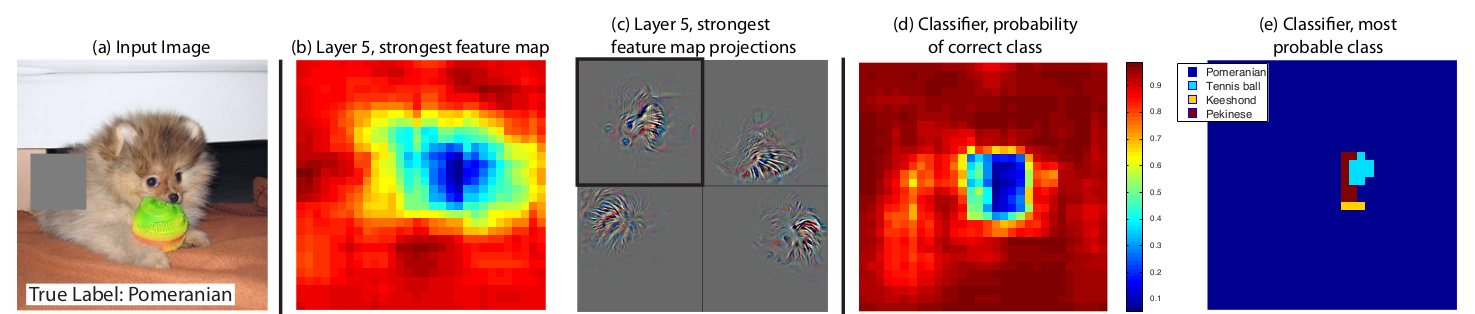
\includegraphics[width=\textwidth]{images/occlusion_sensitivity_map}
    \caption{An illustration of occlusion sensitivity mapping}
    \label{osm}
\end{figure}
    
    
    
 \subsection{Saliency Maps}
 Simonyan et al. \cite{simonyan2013deep} propose two visualization techniques with intents to generate an image which maximizes the class score, and to compute a class-specific saliency map for a given input. The first technique numerically optimizes the input image while the other computes the spatial support of a given class in an input. This work is one of the earliest to leverage saliency maps for the task of weakly-supervised object segmentation. Authors demonstrate the proposed techniques by applying to a deep convnet trained on the ILSVRC-2013 dataset \cite{ILSVRC15}.
 
 \subsubsection{Class Model Visualization}
 The intention of this technique is to numerically generate an image which is representative of the target category with respect to the convolutional net’s class scoring model. This is achieved by finding a L2-regularised image such that the logit $S_{c}$  of a given class c is maximized:
 
 %\begin{equation*}
 	
 %\end{equation*}
 
 where  $\lambda$ refers to the regularization parameter and I is a local optimum, which can be found with help of back propagation. The optimization process uses the mean image of the data set as the initial value. The work also mentions about the prominence of visualizations produced by using logit scores over soft-max/unnormalized class scores.   
    
 \subsubsection{Image-Specific Class Saliency}
  The objective of this technique is to rank pixels of an input image, based on their impact on class scores ($S_c$). Authors provide a couple of interpretations for the class score values/ logits with respect to which saliency maps are created:
  \begin{enumerate}
  	\item A linear approximation of the function learned by  neural network in a local neighbourhood of the input image.
  	\item Higher the saliency associated with a pixel, lesser it needs to be altered in order to increase it respective class’s score.  
  \end{enumerate}

 The derivative of class score with respect to input image is found using back propagation as described by the equation below:
 
  %\begin{equation*}
 
 %\end{equation*}
 
 In order to obtain the saliency map for a multi-channel image, the maximum magnitude of gradient for a given position across channels is used. Class saliency maps thus produced are used as initial points  to compute object segmentation mask using the GraphCut algorithm \cite{boykov2006graph}. Foreground and background portions are considered as Gaussian Mixture Models and the former is estimated from pixels with saliency value higher than the 95\% quantile of the image’s saliency distribution.On the other hand, the latter is estimated from pixels with saliency smaller than 30\% quantile.\\
 The work evaluates its outputs on test split of the data set for the localization task in the ILSVRC-2013 \cite{ILSVRC15} challenge, where it achieves 46.4\% top-5 error in spite of its simplicity.
 In hindsight, apart from the strategy used to reverse the ReLU layer this approach is equivalent to Deconvnet \cite{matthew2014visualizing}.
 
 \subsection{Guided Backpropagation}
 Springenberg et al. proposed a new variant of the deconvolution approach in their work, as a means to analyze their \enquote{All Convolutional Net} architecture, which replaces max-pooling layers by convolutional layers with increased stride. The first objective of this work was to empirically prove the equivalence (in terms of predictive performance) between a max-pooling layer and a convolutional layer with an increased stride. This was achieved by evaluating a custom cnn model with max-pooling layers against its convolutional counterpart on three datasets: CIFAR-10, CIFAR-100 and ILSVRC 2012. In all cases, performances of the all convolutional models were on par with their max pooling counterparts. The second objective was to determine the quality of representations learned by the intermediate layers of the all convolutional neural network models. In order to achieve this, authors proposed a visualization  approach, which can be considered as a slight modification of the Deconvnet \cite{matthew2014visualizing} technique.
 \subsubsection{Back propagation through ReLU}
 One of the most significant difference between Saliency Maps \cite{simonyan2013deep}, Deconvnet \cite{matthew2014visualizing} and Guided backprop \cite{guided_backprop} approaches is the strategy used by these methods to backpropagate gradients through the ReLU layer. 
 
 \begin{itemize}
 	\item Saliency maps approach backpropagates gradients of positions with respective to non-negative activations.
 	%\begin{equation*}
 	%\end{equation*}
 	\item On the other hand, the deconvnet approach allows only positive gradients to flow in reverse direction.
 	%\begin{equation*}
 	%\end{equation*}
 	\item The guided-backprop approach combines the above mentioned methods and masks out values for which at least  one of activation or gradient values is negative. This is performed with an intention to avoid the reverse of negative gradients of neurons which reduce the activation of the target neuronal unit.
	%\begin{equation*}
	%\end{equation*}
 \end{itemize}

Figure b illustrates differences between back propagation strategies with help of an example feature map. 

The term \enquote{guided backpropagation} comes from the use of the additional navigation signal, to selectively back propagate only the positive gradients of the positively activated neuronal units. Though guided backprop was devised to show the learning capability of the all convolutional network architectures, authors show the effectiveness of the technique on the ones with max-pooling units. Guided backprop produced significantly more accurate representation, especially  for higher layers, when compared to Deconvnet and Saliency maps.

\subsection{Deep LIFT}
 Shrikumar et al. propose an attribution technique, which assigns scores to input pixels based on their contribution to change in activation of each neuronal unit with respect to a reference value, which is chosen based on the problem in hand. Authors claim the technique to be computationally inexpensive, and yield meaningful representations in comparison with other methods. Besides, the technique is devised in a way that it is suitable for neural net variants apart from CNN like Recurrent Neural Networks (RNN).\\
 Intuitively, Deep LIFT seeks to explain the deviation in output from some reference output in terms of deviation in input from its respective reference. The motivation to use a reference value, arises from the need to handle the \enquote{saturation problem}.
 \subsubsection{Saturation problem}\label{sec_saturation}
 The saturation problem can be explained intuitively with an example. The figure illustrates a simple neural network whose outputs saturates, when the sum of its inputs ($i_1$ and $i_2$) exceeds 1. Application of any perturbation or gradient based attribution method, to this scenario would lead to creation of undesirable artifacts. For the methods of earlier type, perturbing inputs will not cause any changes in the output. On the other hand, gradient based methods will suffer from lack of gradients in the region where $i_1+i_2 > 1$.
 \subsubsection*{Working}
 Deep LIFT handles this problem by using a reference value, enabling it to backpropagate the importance signal even in zero and discontinuous gradient situations.\\
 The contributions computed by DeepLIFT is analogous to the idea of partial derivatives, except for the fact that change in input is computed with respect to a finite value (activation difference) in the earlier, in contrast to an infinitesimal value in the latter. The concept of \enquote{multipliers} is used to achieve the same.
 %\begin{equation*}
 %\end{equation*}
 $x$ is the input neuron with a difference from reference $\Delta x$, and t is the target neuron with a difference from reference $\Delta t$. C is then the contribution of $\Delta x$ to $\Delta t$.
 Multipliers obey chain rule
  %\begin{equation*}
 %\end{equation*}
 Along with the custom chain rule, the paper also defines a set of rules for neurons of every kind of neural network layer, to assign contribution scores their inputs:
 \begin{itemize}
 	\item Linear rule for linear layers such as the fully-connected and convolutions
 	\item Rescale rule for non-linear transformations such as ReLU, tanh or sigmoid
 	\item Reveal-cancel rule which enables the measurement of marginal effect of having an input over all possible orderings, similar to Shapely values \cite{shapley_values}. 
 \end{itemize}
The technique also takes in to account that a zero contribution could be due to cancellation of positive and negative contributions from a pair of entities. The application of DeepLIFT also depends on the choice of target neuron’s layer, logit or softmax layer in a classifier network, for example. Authors demonstrate the approach by applying it to a CNN trained on MNIST dataset \cite{lecun1998gradient} and an RNN trained on simulated genomic data.\\
The benchmarking on MNIST classifier for various methods was performed on basis of the change in log-odds score, when a selected pixels of a given image belonging to class c0 were erased to convert it to an image of some target class ct. The upper section of figure illustrates the result of masking pixels ordered as the most significant for converting to target classes 3 and 6. As graphically represented in bottom part of figure, DeepLIFT outperformed other backpropagation based methods.

\subsection{Layer-wise Relevance Propagation}

Layer-wise Relevance Propagation (LRP) \cite{lrp} is a complete path attribution method, whose propagation procedure obeys the conservation principle. This ensures that during back propagation, every neuronal unit receives its share of a given network’s output, and continues to equally redistribute it to its predecessor units, until the input layer is reached. Authors of the work claims that the method suffers less from the \enquote{Clever Hans} effect, which occurs when a model produces correct predictions based on wrong features. Besides they show the equivalence between their approach and Taylor decomposition of the network output/activations into contribution scores of individual neurons in lower layers. Further more, they stress upon the fact that their method is computationally less expensive when compared to other approaches like occlusion sensitivity maps and Local Interpretable Model-agnostic Explanations (LIME) \cite{lime}.

Similar to Deep LIFT, LRP operates based on a set of propagation rules, which are framed based on the conservation principle. The rule set defines the logic to propagate relevance scores through different layers, and also provides parameters that can be set based on the application domain, to produce meaningful attribution maps. Although, there are a few variants of LRP each with its own rule set available, only three basic variants were considered for this work and discussed here.

\subsubsection{LRP-0}
In general,  the relationship between the relevance score Rk which is propagated from layer k, onto a neuron in a subsequent lower layer j as Rj can be expressed as follows:

<eqn1>

where $R_j$ is represented as a linear combination of relevance scores from layer $k$, weighted by the  contribution $Z_{jk}$ of neuron $j$ to $k$, normalized with respect to sum of all contribution from the layer to $R_k$.

The contribution $Z_{jk}$ is measured as the activation times its gradient with respect to $R_k$. Substituting the same in eqn 1 gives the following:\\
<eqn2>


The rule also satisfies the fact that 

<Eqn3>

which means to say that a neuron with a zero activation or zero weight association has zero relevance to the output score.

\subsubsection{LRP-$\epsilon$}

LRP-$\epsilon$ is obtained by slightly modifying the LRP-0 rule. The rule incorporates an extra parameter $\epsilon$ in the expression’s denominator, which is responsible for absorbing some relevance from Rk, when it is contradictory. With an increase in $\epsilon$, only the most important explanation factors survive, leading to less noisy explanations. Though, a very high value of $\epsilon$ can result in sparse attribution maps as depicted in Figure \ref{}.

<eqn>

\subsubsection{LRP-$\gamma$}
LRP-$\gamma$ is another enhancement to LRP-0, and it introduces the hyper-parameter $\gamma$, which indicates the weightage given to the positive contributions. With an increase in the value of $\gamma$, negative contributions begin to disappear. There are other rules of choice to adopt such LRP-$\alpha\beta$ enabling the treatment of positive and negative contributions in an asymmetric manner.

<eqn>


Hyperparameters such as $\epsilon$ and $\gamma$ play a vital role in deciding the meaningfulness of attribution maps and are to be set based on repeated experimentation and domain knowledge. Often a composite version of LRP, using all three rules is recommended to obtain human understandable attributions.
Authors recommend to  use LRP-0 for the last layers, as the propagation rule closely approximates the underlying  neural network function. This is desirable in handling those layers where concepts from different classes are closely entangled. LRP-$\epsilon$ is recommended for the middle layers, which are relatively less entangled when compared to the last ones. They claim that LRP-$\epsilon$ effectively filters out spurious variations resulting from weight sharing, and retains the most salient explanation factors. LRP-$\gamma$ is preferred for the lower layers as this rule spreads the propagated relevance score uniformly to features in an uniform manner. 
\section{Layer Attribution Methods}
Layer attribution methods evaluate contribution of each neuronal unit in a given convolutional layer to a model's output. This section discusses three SOTA methods of the category, considered for our work.
\subsection{GradCAM}
\label{sec_gradcam}
Selvaraju et al. propose GradCAM \cite{selvaraju2017grad}, a pixel-attribution technique leveraging the gradients of a given target class with respect to a convolution layer. This approach can be considered as a generalization of CAM for CNNs with fully connected layers. Besides, the technique is applicable to neural network architectures for tasks such as image captioning and visual-question answering. The work also comes up with a means to convert class-agnostic fine grained visualization approaches like Guided-Backprop and Deconvolution to be class-discriminative in nature.\\
Grad-CAM is one of the most widely used approaches in obtaining attribution map based explanations, for neural network models used with medical data. Concisely put, Grad-CAM creates a visualization of which parts of an input image a convolutional layer “looks” for a certain class prediction. The working of Grad-CAM can be described in the following steps:
\begin{enumerate}
	\item Perform a forward pass of the input image through CNN to obtain logit scores for all classes.
	\item  Except for the logit activation of the class of interest, set other activations to zero.
	\item Backpropagate the gradient of the class of interest all the way to the chosen convolutional layer containing k feature maps Ak. $\partial y_c /\partial A_k$
	\item Global pooling: For every feature map, weigh their pixels based on the gradient value, and obtain their weighted mean value scaled by constant Z
	  %\begin{equation*}
	  %\end{equation*}
	where $y_c$ refers to logit score for class c, $A^k$ refers to the $k^{th}$ activation map of dimensions ixj and $\alpha$ refers to the computed weightage.
	\item Obtain the $\alpha$ weighted average of all pooled feature maps and apply a ReLU to filter out negative values, if any present.
	%begin{equation*}
	%end{equation*}
	where Lc refers to the localization map produced by the Grad-CAM for the class of interest c and Ak refers to the kth feature map.
	\item An element-wise multiplication operation is applied on the scaled version (input image dimensions) of Grad-CAM’s maps, and outputs of fine-grained visualization approaches like Guided-Backpropagation and Deconvolution, to obtain fine-grained yet class discriminative visualizations. These combinations are termed as Guided-GradCAM and Guided-Deconvolution approaches respectively. Guided Grad-CAM visualizations are both high-resolution and class-discriminative.
\end{enumerate}
	
	Typically, last convolutional layers of a neural network model are chosen for Grad-CAM as they contain high-level semantics and detailed spatial information \cite{selvaraju2017grad}. This is because the attribution maps produced by the methods becomes progressively worse qualitatively,  as we use earlier convolutional layers which have relatively lesser receptive fields. In a classification network, logit scores of the target class are used for gradient computations. However, any differentiable activation value can be backpropagated. The embedding based Grad-CAM discussed in the section, draws motivation from this fact. In the original implementation of the attribution method, a Rectified Linear Unit (ReLU) function is applied on heat maps, to obtain only regions that positively affect the given prediction. However, to get better insights into prediction decisions, this work uses unfiltered heat maps, which consists of negatively correlated regions as well.\\  
   Authors evaluate the method on three different tasks: weakly-supervised localization, weakly-supervised segmentation and pointing game experiment \cite{zhang2018top}. The approach is also evaluated and benchmarked on its ability to generate discriminative, trust-worthy, faithful and interpretable attribution maps. A couple of neural network models with different architectures (AlexNet \cite{krizhevsky2012imagenet} and VGG-16) are used for evaluation, to determine the method’s performance consistency across architectures.
   Finally, the work also demonstrates the association of a given concept with a neuron, similar to the ones presented in \cite{matthew2014visualizing} and \cite{zhou2014object}.\\
	Authors also demonstrate it use in analyzing failure modes in neural network models and identifying bias in dataset.
	The approach is considered to be computationally in-expensive when compared to perturbation based methods such as LIME or SHapley Additive exPlanations (SHAP)\cite{shap}, yet producing interpretable and discriminative attribution maps.
	
\subsection{HiResolution Class Activation Mapping (HiResCAM)}
	Draelos et. al propose HiResCAM \cite{draelos2020hirescam} as a generalization of CAM, and the method aims to use feature maps of a layer directly for visualization without averaging unlike GradCAM. The authors demonstrate why the gradient averaging step in attribution methods like GradCAM limit them from being reliable to highlight a neural network model’s regions of attention in an image. Besides, they mathematically show the conceptual relationship between HiResCAM and other CAM approaches. The faithfulness of explanations produced by HiResCAM is shown, by conducting certain experiments on natural images whose results were verified using crowd-sourced assessment.\\
	HiResCAM can be seen as a modification of Grad-CAM, as it is primarily designed to address the later’s limitation caused by its averaging step. As described in \ref{sec_gradcam} and illustrated in the figure below, importance weight $\alpha^f$ for a feature map $f$, is computed by computing the mean of gradients over spatial dimensions. However, the process of averaging may cause the final attribution map not highlight locations within the image which the model used to make predictions.\\
	The above figure illustrates the working of GradCAM and HiResCAM methods. Let $s_m$ be the logit score of a CNN model for a given image input, with respect to class $m$. GradCAM computes the derivative $\partial s_m / \partial A$, which yields the gradient for every position of a feature map. The gradients are then averaged to yield ${\alpha_m}^f$ for every map. Following which, the gradient values are multiplied with feature activation values $(\alpha_m^f A^f)$. While HiResCAM also computes  $\partial s_m / \partial A$, they are multiplied directly with feature map activation values leaving out the averaging procedure. Feature map values across channels are then combined as sum to yield the chosen layer’s attribution map. By skipping the averaging procedure, HiResCAM preserves the effect of the gradients across every feature map.\\
	Similar to GradCAM, authors recommend using the last convolutional layers for visualization. Apart from proposing the method, the authors also argue that explaining a model doesn’t correspond to weakly-supervised segmentation, as the objective of the former to reveal the working of the model while the latter is to localize an object of interest. The work reiterates the fact that every explanation method aims to describe different aspects of model. They also suggest the usage of metrics like IOU to evaluate the localization capability of neural network model than leveraging them to evaluate the correctness of an explanation method. HiResCAM aims to produce faithful explanations even if a model’s regions of interest lie outside an object of interest.\\
	The work compares its method with GradCAM by conducting experiments on PASCAL VOC 2012 \cite{pascal-voc-2012} and a custom made dataset of 20 classes with their ground-truth segmentation maps. Results of the benchmarking experiments reveal the following:
	\begin{itemize}
		\item HiResCAM better reflects computations of the model than GradCAM
		\item Humans perceive explanations produced by both the methods differently
	\end{itemize}
	%figure%
\subsection{Full-Grad}
Full-grad \cite{srinivas2019full} is a gradient-based attribution method, which produces saliency map explanations by providing attributions to both the input image and the neuronal units of intermediate layers of a given neural network. The method is layer-agnostic and produces a single attribution map for an input image passed through a network by model, considering different scales of features, starting from pixel-level to high-level features. This makes the method to produce sharper saliency maps than other techniques.\\
Throughout the work, the authors emphasize the importance of a saliency map based explainability method to satisfy two key properties: 
\begin{enumerate}
	\item Completeness: The ability of a saliency map $S(x)$ representation for an input x, to fully encode the computation performed by a function $f(x)$, such that it can be recovered using $S(x)$ and $x$.
	\item Weak dependence: In a piece-wise linear model, $S(x)$ is dependent only on local neighborhood of $x$ in the data space. 
\end{enumerate}
Authors claim that other saliency mapping methods are able to satisfy only either of these properties. This inability arises from  the exclusion of gradient contributions from the bias components of a neural network model. Besides, they also stress on the need for a saliency mapping method to attribute importance to individual (local attribution) and regions of pixels (global attribution) simultaneously. The novelty of this work lies in its ability to simultaneously satisfy both the completeness and weak dependence properties, by considering gradients associated with bias components for producing saliency maps.\\
The following equation expresses the idea that a ReLU neural network with bias b can be approximated as the sum of  input gradients and bias gradients. The bias term b here considers both explicit bias component and implicit bias such as running mean of batch normalization layers. 
	%equation%
	
Figure shows the ability of the Full-grad method to produce meaningful saliency maps by accumulating both bias and input gradients across all hidden layers. The work also provides the rationale behind its ability to be sensitive to saturation scenarios like zero input attribution, and to produce in corrrect input-output mappings in the case of parameter randomization. The method first obtains spatial maps ($R^D$)  for every convolutional filter called neuron-wise maps. Such maps are then aggregated to form layer-wise maps. The layer-wise maps are further processed by rescaling supplemented with an absolute value operation. The following equation mathematically expresses the process: 

	%equation%

The authors evaluate the effectiveness of the method by conducting two quantitative experiments:
\begin{enumerate}
	\item Pixel perturbation: Replace the least salient input pixels for classification with black pixels, and observe the output variation. The lower the variation in salient regions of the attribution maps, the better is a method.
	\item  RemOve And Retrain (ROAR) experiment \cite{hooker2018evaluating}: In this experiment, the top-k pixels highlighted by an attribution method for an entire data set are removed, and the considered classifier is retrained on this modified data set. The attribution method corresponding to the least accurate classifier model is considered to be the best, as it indicates that the method correctly identified the salient pixels.
\end{enumerate}
The work reports that the FullGrad method outperformed the other considered methods (Input-gradients\cite{shrikumar2017learning}, Integrated-gradients \cite{sundararajan2017axiomatic}, Smooth Grad \cite{smilkov2017smoothgrad} and GradCAM \cite{selvaraju2017grad}) in both the experiments. Apart from the quantitative evaluation, the authors also conducted a visual inspection in which they found the method to produce meaningful attribution maps which highlight both a given object’s boundaries and interiors clearly. Figure

\end{document}
